\documentclass[a4paper]{article}

\usepackage[english]{babel}
\usepackage{amsmath}
\usepackage{amssymb}
\usepackage{dsfont}
\usepackage{tikz}
\usetikzlibrary{arrows,automata}
\title{Calculus and Probability Theory\\ Assignment 4}
\author{Christoph Schmidl\\
s4226887\\
Informatica\\
c.schmidl@student.ru.nl\\
Exercise Teacher: Gergely Alp\'{a}r}

\date{\today}

\begin{document}
\maketitle

\begin{enumerate}

\item (\textbf{26 points}) Evaluate the following definite integrals. (If neccessary, round to two decimal places.).\\

\begin{enumerate}
	\item[(a)] $\int_1^4(x + 3 \sqrt{x} + 2) \; dx$;\\
	\textbf{Solution:}
	
\begin{align*}
	\int_1^4(x + 3 \sqrt{x} + 2)dx &= \int x \; dx + 3 \int x^\frac{1}{2} \; dx + \int 2 \; dx \\
	&= \frac{1}{2}x^2 + 3 \cdot \frac{2}{3}x^\frac{3}{2} + 2x \Bigg]_1^4 \\
	&= \frac{1}{2}x^2 + 2x^\frac{3}{2} + 2x \Bigg]_1^4\\
	&= \frac{1}{2}x^2 + 2 \sqrt{x^3} + 2x \Bigg]_1^4 \\
	&= (\frac{1}{2}4^2 + 2 \sqrt{4^3} + 2 \cdot 4) - (\frac{1}{2}1^2 + 2 \sqrt{1^3} + 2 \cdot 1) \\
	&= 32 - 4 \frac{1}{2} \\
	&= 27.5
\end{align*}	
	
\newpage	
	
	
	\item[(b)] $\int_1^{16}(4x^{\frac{7}{3}} - \sqrt[4]{x} + \frac{\pi}{x}) \; dx$;\\
	\textbf{Solution:}
	
\begin{align*}
	\int_1^{16} (4x^\frac{7}{3} - \sqrt[4]{x} + \frac{\pi}{x}) \; dx &= \int 4x^\frac{7}{3} \; dx - \int \sqrt[4]{x} \; dx + \int \frac{\pi}{x} \; dx \\
	&= 4 \int x^\frac{7}{3} \; dx - \int x^\frac{1}{4} \; dx + \pi \int \frac{1}{x} \; dx \\
	&= 4 \cdot \frac{3}{10}x^\frac{10}{3} - \frac{4}{5}x^\frac{5}{4} + \pi \cdot \ln(x) \Bigg]_1^{16} \\
	&= \frac{12}{10}x^\frac{10}{3} - \frac{4}{5}x^\frac{5}{4} + \pi \cdot \ln(x) \Bigg]_1^{16} \\
	&= \frac{12}{10} \sqrt[3]{x^{10}} - \frac{4}{5} \sqrt[4]{x^5} + \pi \cdot \ln(x) \Bigg]_1^{16} \\
\end{align*}	
	
\begin{align*}
&= (\frac{12}{10} \sqrt[3]{16^{10}} - \frac{4}{5} \sqrt[4]{16^5} + \pi \cdot \ln(16))-(\frac{12}{10} \sqrt[3]{1^{10}} - \frac{4}{5} \sqrt[4]{1^5} + \pi \cdot \ln(1))\\
&= 12368.63823 - 0.4\\
&\approx 12368.24
\end{align*}	
	
	
	
	
	\item[(c)] $\int_{-2}^2(e^{5x-1}) \; dx$. (Hint: Apply substitution).\\
	\textbf{Solution:}\\

\begin{align*}
	\int_{-2}^2(e^{5x-1}) \; dx \\
\end{align*}

$Let \; u = 5x - 1$\\ 

$\frac{du}{dx} = 5 \rightarrow 5dx = du$	

\begin{align*}
	\int_{-2}^2(e^{u}) \; \frac{du}{5} &= \frac{1}{5}\int e^u \; du = \frac{1}{5} e^u \Bigg]_{-2}^2 = \frac{1}{5}e^{5x-1} \Bigg]_{-2}^2\\
\end{align*}
	
\begin{align*}
\frac{1}{5}e^{5x-1} \Bigg]_{-2}^2 &= (\frac{1}{5}e^{5(2)-1})-(\frac{1}{5}e^{5(-2)-1})\\
&\approx 1620.62
\end{align*}	
	
	
	
\end{enumerate}


\item (\textbf{40 points}) Determine the indefinite integrals by applying the substitution method.

\begin{enumerate}
	\item[(a)] $\int \sqrt{x + 1} \; dx$. Verify the result.\\
	\textbf{Solution:}\\	
	
	
\begin{align*}
	\int \sqrt{x + 1} \; dx
\end{align*}	
	
$Let \; u = x+1$\\ 

$\frac{du}{dx} = 1 \rightarrow 1dx = du$

\begin{align*}
\int \sqrt{u} \; du &= \int u^\frac{1}{2} \; du\\
&= \frac{2}{3}u^\frac{3}{2} + C\\
&= \frac{2}{3}(x+1)^\frac{3}{2} + C
\end{align*}	
	
\textit{Control:}

\begin{align*}
	\frac{d}{dx} (\frac{2}{3} (x + 1)^\frac{3}{2} + c) &= \frac{d}{dx}(\frac{2}{3}(x + 1)^\frac{3}{2})\\
	&= \frac{2}{3} \frac{d}{dx} (x+1)^\frac{3}{2}
\end{align*}

$Let \; u = x+1$\\ 

$\frac{d}{du} u^\frac{3}{2} = \frac{3}{2}u^\frac{1}{2} = \frac{3 \sqrt{u}}{2}$

\begin{align*}
	\frac{2}{3} \frac{3 \sqrt{x+1} \frac{d}{dx}(1 + x)}{2} = \frac{2}{3} \frac{3 \sqrt{x + 1}}{2} = \frac{\frac{6}{3}\sqrt{x + 1}}{2} = \sqrt{x + 1}
\end{align*}
	
	\item[(b)] $\int \sin(2x - 3) \; dx$\\
	\textbf{Solution:}\\
	

\begin{align*}
\int \sin(2x - 3) \; dx
\end{align*}	
	
$Let \; u = 2x - 3$\\ 

$\frac{du}{dx} = 2 \rightarrow 2dx = du \rightarrow dx = \frac{1}{2}du$	

\begin{align*}
\int \frac{1}{2}\sin(u) \; du &= \frac{1}{2} \int \sin(u) \; du\\
&= \frac{1}{2} \cdot (- \cos(u)) + C
&= \frac{1}{2} \cdot (- \cos(2x - 1)) + C\\
&= -\frac{1}{2} \cos(2x-3) + C
\end{align*}	
	
	\item[(c)] $\int 5x \cdot \cos(3x^2 + 5) \; dx$\\
\textbf{Solution:}\\	
	
\begin{align*}
\int 5x \cdot \cos(3x^2 + 5) \; dx
\end{align*}	

$Let \; u = 3x^2 + 5$\\ 

$\frac{du}{dx} = 6x \rightarrow 6xdx = du \rightarrow dx = \frac{1}{6}xdu$	
	
\begin{align*}
5 \int x \cdot \cos(u) \; du &= \frac{5}{6} \int \cos(u) \; du\\
&= \frac{5}{6}\sin(u) + C\\
&= \frac{5}{6} \sin(3x^2 + 5) + C
\end{align*}		
	
	
	\item[(d)] $\frac{1}{3} \int 3^{x^4} \cdot x^3 \; dx$. Verify the result.\\
	\textbf{Solution:}\\
	
\begin{align*}
\frac{1}{3} \int 3^{x^4} \cdot x^3 \; dx
\end{align*}	
	
$Let \; u = x^4$\\ 

$\frac{du}{dx} = 4x^3 \rightarrow 4x^3dx = du$	

\begin{align*}
	\frac{1}{3} (\frac{1}{4} \int 3^u \cdot 1 \; du) &= \frac{1}{3}(\frac{1}{4} (\frac{1}{\ln(3)}3^u) + C)\\
	&= \frac{1}{3}( \frac{1}{4}\frac{3^u}{\ln(3)})\\
	&= \frac{1}{3} (\frac{1}{4} \frac{3^{x^4}}{\ln(3)})\\
	&= \frac{1}{3} (\frac{3^{x^4}}{\ln(81)})
\end{align*}
	
	
\textit{Control:}	
	
\begin{align*}
	\frac{d}{dx}(\frac{3^{x^4}}{\ln(81)})
\end{align*}	
	
$Let \; u = x^4$\\ 

$\frac{du}{dx} = 4x^3$\\

$\frac{d}{du} 3^u = 3^u \ln(3)$	
	
\begin{align*}
	\frac{4x^3 3^{x^4} \ln(3)}{\ln(81)} = \frac{1}{4} 4x^3 3^{x^4} = 3^{x^4} \cdot x^3
\end{align*}	
	
Putting back the leading $\frac{1}{3}$	before the integral and we get back to the original.\\
	
	
	\item[(e)] $\int \frac{2}{\sqrt{1 - (2x + 5)^2}}dx$. (Hint: arcsin).\\
	\textbf{Solution:}\\
	
\begin{align*}
	\int \frac{2}{\sqrt{1 - (2x + 5)^2}} \; dx &= 2 \int \frac{1}{\sqrt{1 - (2x + 5)^2}} \; dx
\end{align*}	
	
$Let \; u = 2x+5$\\ 

$\frac{du}{dx} = 2 \rightarrow 2dx = du \rightarrow du = \frac{1}{2}du$	

\begin{align*}
	\int \frac{1}{\sqrt{1 - u}^2} \; du &= \arcsin(u) + C\\
	&= \arcsin(2x + 5) + C
\end{align*}	
	
	\item[(f)] $\int \frac{4x - 10}{\sqrt{1 - (4x^2 - 20x + 25)^2}}dx$ (Hint: again?)\\
	\textbf{Solution:}\\
	
\begin{align*}
	\int \frac{4x - 10}{\sqrt{1 - (4x^2 - 20x + 25)^2}}dx &= \int 4x - 10 \frac{1}{\sqrt{1 - (4x^2 - 20x + 25)^2}}
\end{align*}	
	
$Let \; u = 4x^2 - 20x + 25$\\ 

$\frac{du}{dx} = 8x - 20 \rightarrow 8x - 20dx = du \rightarrow du = \frac{1}{8x - 20dx}$		
	
	
\begin{align*}
	\int \frac{4x - 10}{8x - 20} \frac{1}{\sqrt{(1 - u)^2}} \; du &= \int \frac{1}{2} \frac{1}{\sqrt{(1 - u)^2}} \; du\\
	&= \frac{1}{2} \int \frac{1}{(1-u)^2} \; du\\
	&= \frac{1}{2} \arcsin(u) + C\\
	&= \frac{1}{2} \arcsin(4x^2 - 20x + 25) + C
\end{align*}	
	
	
\end{enumerate}


\item (\textbf{10 points}) Given the function $f(x) = -x^2 + 8x - 7$. What is the area under the curve of $f$ between the zeros of the function?\\
\textbf{Solution:}\\

1. Determine the roots of the function\\

Using the ABC-formula: 

\begin{equation}
	ax^2 + bx + c = 0 \Rightarrow x = \frac{-b \pm \sqrt{b^2 - 4ac}}{2a} \notag
\end{equation}

$x = \frac{-8 \pm \sqrt{8^2 - 4 \cdot (-1) \cdot (-7)}}{-2} = \frac{-8 \pm \sqrt{64 - 28}}{-2} = \frac{-8 \pm \sqrt{36}}{-2}= \frac{-8 \pm 6}{-2}$\\

$x_1 = 1$\\
$x_2 = 7$\\


2. Take the roots for the definite integral\\

\begin{align*}
\int_1^7(-x^2 + 8x -7) \; dx &= -\frac{1}{3}x^3 + 4x^2 - 7x \Bigg]_1^7\\
&= (-\frac{1}{3}7^3 + 4 \cdot 7^2 - 7 \cdot 7) - (-\frac{1}{3}1^3 + 4 \cdot 1^2 - 7 \cdot 1)\\
&= (-\frac{1}{3} \cdot 343 + 4 \cdot 49 - 49) - (-\frac{1}{3} + 4 - 7)\\
&= -\frac{343}{3} + 147 + \frac{1}{3} + 3\\
&= - 114 + 147 + 3\\
&= 36
\end{align*}
\newpage

The area under the curve $f$ between the zeros of the function (namely 1 and 7) is 36.\\


\begin{figure}[ht]
	\centering
  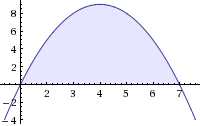
\includegraphics[width=0.5\textwidth]{area.png}
\end{figure}	

\item (\textbf{24 points}) Let $f(x) = \ln x$. Solve the problems below in order.\\

\begin{enumerate}
	\item[(a)] Find $b \in \mathbb{R}$ such that $f(b) = 1$\\
	\textbf{Solution:}\\
	
I already know by heart that $ln(e) = 1$.\\ So, $b = e$\\
	
	
	
	
	\item[(b)] Determine the equation of the tangent line at the point $(b,1)$.\\
	\textbf{Solution:}\\
	
1. Find the derivative of this function to find the equation for the slope of the curve.\\

$f'(x) = \frac{1}{x}$\\
	
2. Plug the x-value of this point into the derived function to find the slope of the curve at that point.\\

$y = \frac{1}{e}$\\
	
	
3. Equation of the tangent line at the point (e,1)\\

$y - 1 = \frac{1}{e}(x - e)$\\
	
	
\begin{figure}[ht]
	\centering
  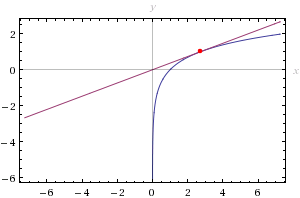
\includegraphics[width=0.6\textwidth]{tangent.png}
\end{figure}	
	
\newpage	
	
	
	
	
	\item[(c)] Let this line intersect the x-axis at $a$. What is the area of the triangle with the following vertices:\\
	$(a,0),(b,1),(b,0)$\\
	\textbf{Solution:}\\
	
Determine line intersect with x-axis\\

\begin{align*}
 	y - 1 &= \frac{1}{e}(x - e)\\
 	y &= \frac{1}{e}(x - e) + 1\\
 	0 &= \frac{1}{e}(x - e) + 1\\
 	x &= 0 \rightarrow a = 0
\end{align*}	
	
	
	
We get a triangle with the following vertices: (0,0), (e,1), (e,0)	
	
\begin{figure}[ht]
	\centering
  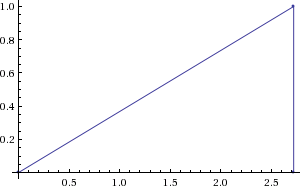
\includegraphics[width=0.6\textwidth]{triangle.png}
\end{figure}	
	
	
Because this gives us a right-angled triangle, we can use the following formula:	
	
\begin{align*}
A = \frac{e \cdot 1}{2} = \frac{e}{2}
\end{align*}	
	
The area of the triangle is $\frac{e}{2}$
	
	
	\item[(d)] Someone tells you that ($x \ln x - x)' = \ln x$. Verify whether it is true.\\
	\textbf{Solution:}\\
	
\begin{align*}
	\frac{d}{dx}(x \ln x - x) &= -1 + \frac{d}{dx} (x \ln x)\\
	&= -1 + \ln x \cdot 1 + x \frac{d}{dx} (\ln x)\\
	&= -1 + \ln x + \frac{1}{x}x\\
	&= -1 + \ln x + \frac{x}{x}\\
	&= \ln x
\end{align*}	
	
	
	\item[(e)] Determine $\int_1^b \ln x \; dx$.\\
	\textbf{Solution:}\\
	
We already know from (d) that $(x \ln x - x)' = \ln x$, so we just have to plug in the values.\\


\begin{align*}
	\int_1^e \ln x \; dx &= x \ln x -x \Bigg]_1^e\\
	&= (e \ln(e) - e)-(1 \cdot \ln(1) - 1)\\
	&= (e \cdot 1 - e) - (1 \cdot 0 - 1)\\
	&= 1
\end{align*}	
	
\begin{figure}[ht]
	\centering
  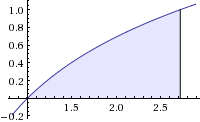
\includegraphics[width=0.4\textwidth]{e.png}
\end{figure}	
	
The area is 1.	
	
	
\end{enumerate}




	
\end{enumerate}

\end{document}
